\documentclass{article}
\usepackage[utf8]{inputenc}
\usepackage{pdfpages}
\usepackage{graphicx}
\usepackage[export]{adjustbox}
\usepackage{caption}
\usepackage[official]{eurosym}
 
\newcommand{\marginnote}[1]{\mbox{}\marginpar{\tiny\raggedright{$>$  #1}}}
\newcommand{\luchnote}[1]{\mbox{}\marginpar{\tiny\raggedright{\textbf{Luch:}  #1}}}
 
 
\title{Scorify: Live score generation for instruments and electronics.}

\date{}
 
\begin{document}
 
\maketitle

\abstract{I propose a system of graphic notation for both instrument and electronics with the capability to combine realtime and non-realtime composition. Primarily intended for mixed media, this project attempts to bridge instrumental and electronic notation. Using Pure Data's ``data structures,'' combined with networked computers, this project reduced not only the notational gap between instruments and electronics, but also brings forth realtime composition based in audio feature extraction.}

\section{Concept}

\noindent I propose a system of graphic notation for both instrument and electronics with the capability to combine realtime and non-realtime composition. This system relies on Pure Data's ``data structures'' for its graphical interface. This allows for both manual and automatic editing. This is to say that the composer can edit with the cursor each element, as lines or dots on a graphical canvas, like in other traditional graphic notation software (i.e., HighC). However, the graphical environment can be edited automatically or generated in realtime, either by constructing the algorithmia from within Pd, or by sending values via TCP/IP from other programs (e.g., Supercollider, MaxMSP, etc.) Furthermore, scores can be edited and stored for further use, for example, as in a generation of a database of scores which can be read in different orders or combinations. \\

\noindent This project is primarily meant for mixed media, but it can easily be used for acousmatic music. At heart, this graphical interface attempts to bridge instrumental and electronic notation. In general, electronic instrument notation is essentially parametric. Thus, by rendering parametric scores for performers, the notational gap is reduced, and in compositional terms this means more connection between the sonic ideas and their performativity. By doing this, I attempt to distill some of the bagage traditional notation presents to performances and to composition, in order to bring closer the sonic and gestural worlds of speakers and instruments. When working for playes, thus, scores can be sent to different computers in a network (TCP/IP type of connections), or to different screens connected to the same computer, and the electronic instruments can also receive and read the score.\\

\noindent Since the electronic instrument is so versatile and varied, I only chose a simple example from Pure Data's audio examples, to quickly show how the system is working as of now. In more complex situations, for example, in a spatial music context, the graphical interface can be used to control azimuth, elevation, etc., to work with different panning trajectories.  \\

\noindent One of the major drawbacks this project currently has is the amount of restrictions which are imposed by Pure Data's data structures functionality, which in itself depends on the Tk graphical system. However, since the Pd developer community is working on this field, I am confident this will become a much more fluent graphical environment algogether. \\

\noindent One of the major advantages this system pushes forward is the live score generation based on live analysis of each sound source. Using William Brent's suite of externals for realtime feature extraction (TimbreID) it is possible to carry out such analysis in order to shape the development of the music. This is to say that each player, including the electronic instrument, will have their own analysis chain, from which a set of algorithmic rules can be prescribed in order for the next page to be generated. Then, for example, each page of instrument A would depend on the previous page either of instrument A or of instrument B. Thus, the overall arch of the sonic experience would come to be an emergent phenomenon that depends on the moment of playing, subject to the contingencies of such moment. By pushing forward a different conceptualization of the composer and its authority, this project is simultaneously framed and unframed in an-archic compositional practice. \\

\subsection{The Software}

\begin{enumerate}

\item Puredata (http://msp.ucsd.edu)

\item Scorify (https://github.com/fdch/scorify)

\end{enumerate}


\section{Example}


\begin{figure}[htbp]
\begin{center}
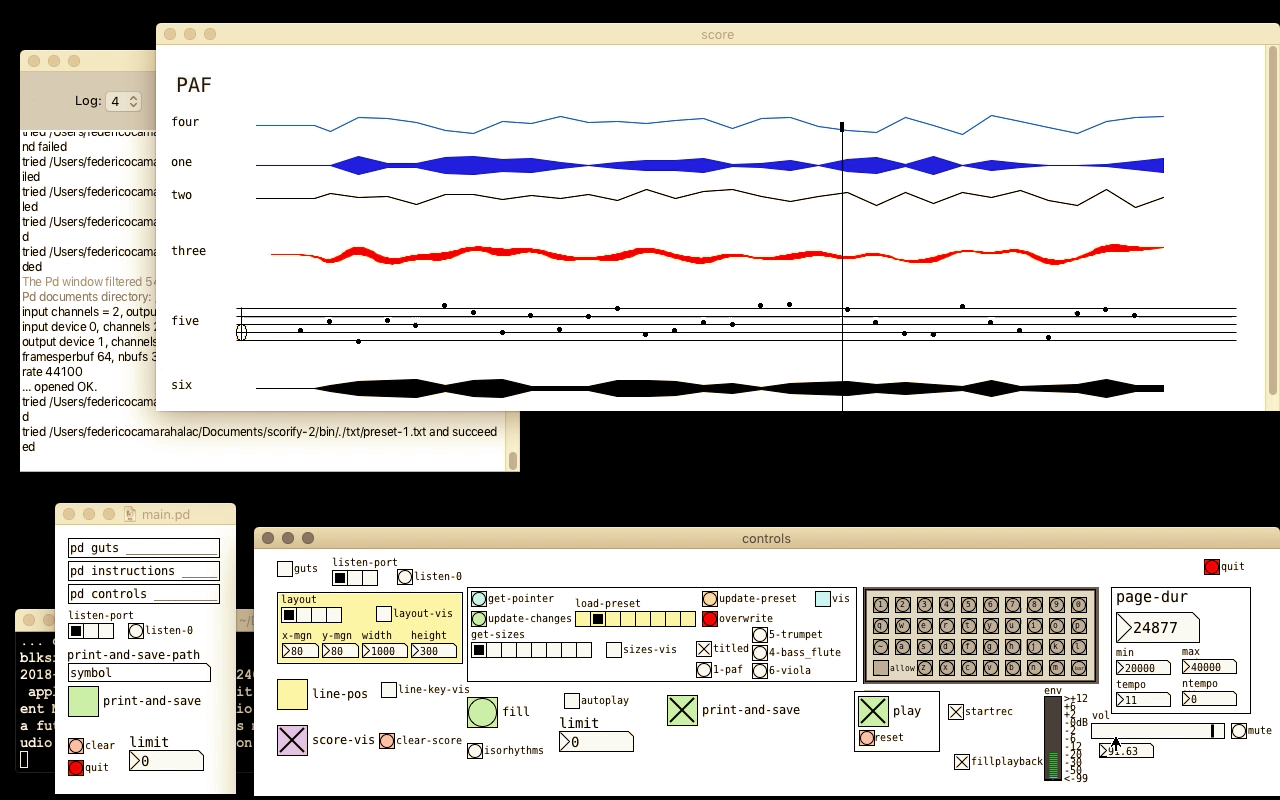
\includegraphics[width=\textwidth]{screenshot.png}
\caption{screenshot}
\label{fig:screenshot}
\end{center}
\end{figure}



\end{document}
